\documentclass[utf8]{frontiersSCNS}
\usepackage{gensymb}
\usepackage{url,hyperref,lineno,microtype,subcaption}
\usepackage[onehalfspacing]{setspace}

\linenumbers
\usepackage{wasysym} % provides \DH, \dh, \Thorn, \thorn
% Leave a blank\usepackage{amsmath}
%\DeclareMathOperator{\sign}{sign} line between paragraphs instead of using \\

\usepackage{booktabs}
\usepackage{multirow}
\usepackage{siunitx} %for SI units
\usepackage{lscape} % for landscape table

\def\keyFont{\fontsize{8}{11}\helveticabold }
\def\firstAuthorLast{Balasubramanian {et~al.}} %use et al only if is more than 1 author
\def\Authors{Suryanarayanan Balasubramanian\,$^{1}$, Roger Waser\,$^{2}$, Martin Hoelzle\,$^{1}$}
\def\Address{$^{1}$University of Fribourg, Department of Geosciences, Fribourg, Switzerland $^{2}$University of
Applied Sciences and Arts, Luzern, Switzerland} \def\corrAuthor{Suryanarayanan Balasubramanian}

\def\corrEmail{suryanarayanan.balasubramanian@unifr.ch}


\begin{document}
\onecolumn
\firstpage{1}

\title[Scheduling AIR fountains]{Fountain scheduling for efficient artificial ice reservoirs (Icestupas): theory and
practice }

\author[\firstAuthorLast ]{\Authors}
\address{}
\correspondance{}

\extraAuth{}

% \maketitle

\begin{abstract}
  To construct artificial ice reservoirs (AIRs) with limited water resources requires a high water use
  efficiency (WUE). This can be achieved by the precise scheduling of the fountain water spray taking into
  account the AIRs response to weather conditions. We solve the corresponding optimization problem, i.e. finding
  the ideal discharge rate for maximum WUE by two approaches differing in operation costs which offer
  straightforward application facilities . The automation software uses a simplified equation with 6
  coefficients that capture the influence of temperature, humidity, wind and solar radiation variations on the
  freezing rate. Historical meteorological data of the site is required to calculate these 6 coefficients. The
  automated AIR had a WUE three times more than the manual AIR. These results support the use of the model in
  practice. \tiny \keyFont{ \section{Keywords:} icestupa, water storage, climate change adaptation,
  geoengineering, nature based solution} %All article types: you may provide up to 8 keywords; at least 5 are
mandatory. \end{abstract}

\section{Introduction}
Artificial Ice Reservoirs (AIRs) have recently received much attention in the light of increasing users,
especially in semi-arid and arid mountain regions facing limited water availability and at the same time
increased water needs. However, their water use efficiency (WUE) is very poor. 

Fountain scheduling methods are one option for reducing watering volumes for AIR construction systems and, at
the same time, increase WUE. The goal of fountain scheduling is to make the most efficient use of water by
spraying the right amount of water at the right time, making sure water is available when the AIR surface can
freeze it. Scheduling maximizes AIR WUE by minimizing fountain waste water.  

Proper fountain scheduling requires answers to two questions: (a) When should the water be turned on and off?
(b) How much water should be sprayed? Question (a) can be answered accurately based on the sign of the surface
energy balance. However, question (b) requires information on both the magnitude of the energy balance and the
fountain spray radius over which this energy balance acts.  

However, efficient AIR construction is challenging, due to the many factors that should be considered, including
weather, water source, fountain characteristics and operation costs. Since this technology is currently being
used by subsistence farmers, we propose two different methods of fountain scheduling based on operation costs
that can be classified as static or dynamic. According to the static approach the total amount of water for AIR
construction is allocated without specifying its temporal distribution along the accumulation period. By
contrast, in the dynamic approach water is allocated at specific time steps along the accumulation period in
order to achieve even higher WUE.

The static approach requires only a fountain and pipeline system which are readily available to farmers. For
fountain scheduling, one just needs to know the recommended freezing rate of the construction location and
measure the spray radius of the fountain used. Given these materials and information, the fountain scheduling
can be achieved by tuning the discharge rate according to the recommended freezing rate and switching on the
fountain between sunset to sunrise. However, this approach is likely to yield lower WUE and ice volumes since it
does not take advantage of the variations in the freezing rate and the freezing time windows during the day.

Along with the materials required for the static approach, the dynamic approach requires a sophisticated
automation system attached to the fountain pipeline. The additional energy required for the automation system
can be obtained via solar panels. Such a system requires minimal manual intervention compared to the static
approach. Since this system makes real-time adjustments of the fountain discharge rate it is likely to produce
much higher WUE and ice volumes compared to the static method. However, the setup cost of such a system could be
double that of the static method.

Knowledge of surface freezing rates is important for the correct assessment and management of these water
reservoirs. Surface freezing rates can be calculated by means of two different approaches: physical
energy-balance models and empirical models. The former may be defined as a model in which each of the relevant
energy fluxes at the AIR surface is computed from physically based calculations using direct measurements of
the necessary meteorological variables, and the freezing rate is calculated as the sum of the individual fluxes
scaled with the AIR surface area during the accumulation period. The latter may be defined as a model in which
the freezing rate is calculated from an empirical formula in which air temperature is the primary measured
input variable, although additional input variables, such as relative humidity, wind speed and incoming solar
radiation, may be incorporated through parametrizations based on time and location. Empirical models
have been widely used for both glaciological and hydrological applications due to their parsimony in data
requirement in comparison with the more sophisticated energy-balance models.

The main aim of this study is to develop a freeze model with lower data requirement than the energy-balance
model presented in \cite{Balasubramanian_2022} that can be used to determine the recommended discharge rate of
any construction location. This is achieved by:

\begin{itemize}

  \item incorporating assumptions that reduce the input requirements of \cite{Balasubramanian_2022} model to
    variables readily available in reanalysis products.
  \item developing a linear equation with the temperature-dependent energy sources through linear regression and
    the solar-dependent energy sources using the coordinates and the altitude of the construction location. 

\end{itemize}


\section{Study Sites and data}

\section{Automation software}
The objective of the automation software is to estimate the freezing rate given minimal weather, fountain and
location information. From \cite{Balasubramanian_2022}, the freezing rate of the AIR can be represented as: 

\begin{equation}
	 \frac{\Delta M_{freeze}}{\Delta t}  = (q_{SW} + q_{LW} + q_{L} + q_{S} + q_{F} + q_{G}) * A_{cone}
	\label{eqn:freeze}
\end{equation}

We simplify the above equation with several assumptions relating to each of its components. We tend to use
assumptions that underestimate the associated freezing rate to optimise for WUE. Further description of our
assumptions are described in the Appendix. Below, we summarise the list of assumptions used:

\begin{itemize}
  \item $A_{cone}$ : The area of the conical AIR is approximated to the area of its circular base produced through the fountain spray
radius $r_F$. This assumption underestimates the surface area of the AIR during the accumulation period and
thereby underestimates the freezing rate.

  \item $q_{SW}$: The direct and diffuse components of shortwave radiation are estimated from the coordinates,
    altitude and time using the PVLIB module.

  \item $q_{LW}$: 

  \item $q_{S}$:

  \item $q_{L}$:

  \item $q_{F}$:

  \item $q_{G}$:

\end{itemize}


The area of the conical AIR is approximated to the area of its circular base produced through the fountain spray
radius $r_F$. Therefore, the surface area can be determined using

\begin{equation} A_{cone} =\pi \cdot r_{F}^2 \label{eq:Area} \end{equation}

Admittedly, this assumption underestimates the surface area of the AIR during the accumulation period and
thereby underestimates the freezing rate.

We approximate the energy balance at the surface of an AIR by a one-dimensional description of energy fluxes as
used in \cite{Balasubramanian_2022}:


Upward and downward fluxes relative to the ice surface are positive and negative, respectively. The first
term represents the energy change used for freezing the fountain water and melting the ice respectively.
$q_{SW}$ is the net shortwave radiation; $q_{LW}$ is the net longwave radiation; $q_{L}$ and $q_{S}$ are the
turbulent latent and sensible heat fluxes. 

The software assumes $T_{ice} = 0 \degree C$ and therefore ignores the temperature change flux $q_{T}$, fountain
heat flux $q_{F}$ and ground heat flux $q_{G}$. All these assumptions overestimate the freezing rate.

Furthermore, we the rest of the energy balance components based on their air temperature and solar
radiation dependence. Namely, $q_{LW}$, $q_{L}$ and $q_{S}$ contribute to temperature induced freeze rate and
$q_{SW}$ contributes to solar radiation induced melt rate during the accumulation period.  Particularly,

For the static method, we only need to determine the night freezing rates whereas for the dynamic approach we
also need to account for the day melt during the accumulation period.

\subsubsection{Temperature induced freeze rate } \label{sec:Temp_rate}

\begin{equation}
	 f(T_a, RH, v_a; alt) = q_{LW} + q_{L} + q_{S}
	\label{eqn:Temp_rate}
\end{equation}

\subsubsection{Radiation induced melt rate \texorpdfstring{$q_{SW}$}{Lg}}
\label{sec:SW}
\begin{equation}
	 g(time) = q_{SW}
	\label{eqn:Temp_rate}
\end{equation}

\subsection{Automation equation}

Using the above simplifications, we can now approximate $q_{LW}$, $q_{L}$ and $q_{S}$ using just temperature,
relative humidity and wind speed. 


\begin{subequations}

	\begin{align}
		\label{eqn:SW}
    \frac{q_{SW} \cdot A_{cone} \cdot \Delta t}{L_F} & = \frac{amp}{(\sigma \sqrt{2\pi})} \cdot
    exp\left(\frac{-(time-\mu)^2}{2\sigma^2}\right) \\
		\label{eqn:T}
    \frac{(q_{LW} + q_{S} + q_{L}) \cdot A_{cone} \cdot \Delta t}{L_F} & = a \cdot T_a + b \cdot RH + c \cdot v_a +
  d \\
		\label{eqn:auto}
    \frac{q_{total} \cdot A_{cone} \cdot \Delta t}{L_F} & = \frac{amp}{(\sigma \sqrt{2\pi})} \cdot
    exp\left(\frac{-(time-\mu)^2}{2\sigma^2}\right) + a \cdot T_a + b \cdot RH + c \cdot v_a + d
	\end{align}
\end{subequations}

The first term in Eqn. \ref{eqn:auto} is the expected freezing/melting rate of the AIR. Hence the automation
equation can now be formulated as:

\begin{subequations}
	\begin{align}
		\label{eqn:SW}
  \frac{q_{total} \cdot A_{cone} \cdot \Delta t}{L_F} & = \left\{ \begin{array}{ll}
		\frac{\Delta M_{water}}{\Delta t} & \textit{ if } q_{total} > 0 \\
		\frac{-\Delta M_{ice}}{\Delta t} & \textit{ if } q_{total} \leq 0
	\end{array} \right. \\
  f(time;T_a;RH;v_a) & = \left\{ \begin{array}{ll}
		\frac{amp}{(\sigma \sqrt{2\pi})} \cdot
    exp\left(\frac{-(time-\mu)^2}{2\sigma^2}\right) + a \cdot T_a + b \cdot RH + c \cdot v_a + d
    & \textit{ if } \frac{\Delta M_{ice}}{\Delta t} > d_{crit} \\
		0 & \textit{ if } \frac{\Delta M_{ice}}{\Delta t} \leq d_{crit}
	\end{array} \right.
	\end{align}
\end{subequations}

% Similarly, the diurnal variation of the shortwave radiation can be captured via a gaussian equation. However,
% the seasonal variations in the amplitude of the solar radiation are poorly captured by such an equation. Since,
% typical AIRs have a construction period spanning less than 3 months, we can ignore the seasonal variations of
% solar radiation. Therefore, the net shortwave radiation $q_{SW}$ is computed as follows: 

% , the automation equation is composed of two parts namely, (a) linear and (b) gaussian equation. (a)
% approximates the influence of temperature, wind speed and humidity on the expected freezing rate. (b)
% approximates the contribution of solar radiation on the expected freezing rates.

% \begin{landscape}
% \begin{table}[]
% \centering
% \caption{}
% \label{tab:my-table}
% \begin{tabular}{@{}lllll@{}}
% \toprule
% \textbf{Module name} & \textbf{Symbol} & \textbf{Full eqn} & \textbf{Simplified eqn} & \textbf{Assumptions} \\ \midrule
% \multicolumn{1}{|l}{Surface Area}        & $A_{cone}$ &  & \pi \cdot r_{F}^2 & \multicolumn{1}{l|}{} \\ \midrule
% \multicolumn{1}{|l}{Shortwave Radiation} & $q_{SW}$ &  & (1- \alpha_{ice}) \cdot ( (1- cld) \cdot SW_{global} \cdot f_{cone} + cld \cdot SW_{global}) & \multicolumn{1}{l|}{} \\ \midrule
% \multicolumn{1}{|l}{Longwave Radiation}  & $q_{LW}$ &  & \sigma \cdot \epsilon_a \cdot {(T_a+ 273.15)}^4 -\sigma \cdot \epsilon_{ice} \cdot {273.15}^4 & \multicolumn{1}{l|}{} \\ \midrule
% \multicolumn{1}{|l}{Sensible Heat}       & $q_{S}$ &  &  & \multicolumn{1}{l|}{} \\ \midrule
% \multicolumn{1}{|l}{Latent Heat}         & $q_{L}$ &  &  & \multicolumn{1}{l|}{} \\ \bottomrule
% \multicolumn{1}{|l}{Temperature heat flux} & $q_{T}$ &  & 0 & \multicolumn{1}{l|}{} \\ \bottomrule
% \multicolumn{1}{|l}{Fountain discharge heat flux} & $q_{F}$ &  & 0 & \multicolumn{1}{l|}{} \\ \bottomrule
% \multicolumn{1}{|l}{Ground heat flux}    & $q_{G}$ &  & 0 & \multicolumn{1}{l|}{} \\ \bottomrule
% \end{tabular}
% \end{table}
% \end{landscape}
\section{Automation hardware}

\section{Results}

\begin{figure}
	\begin{center}
		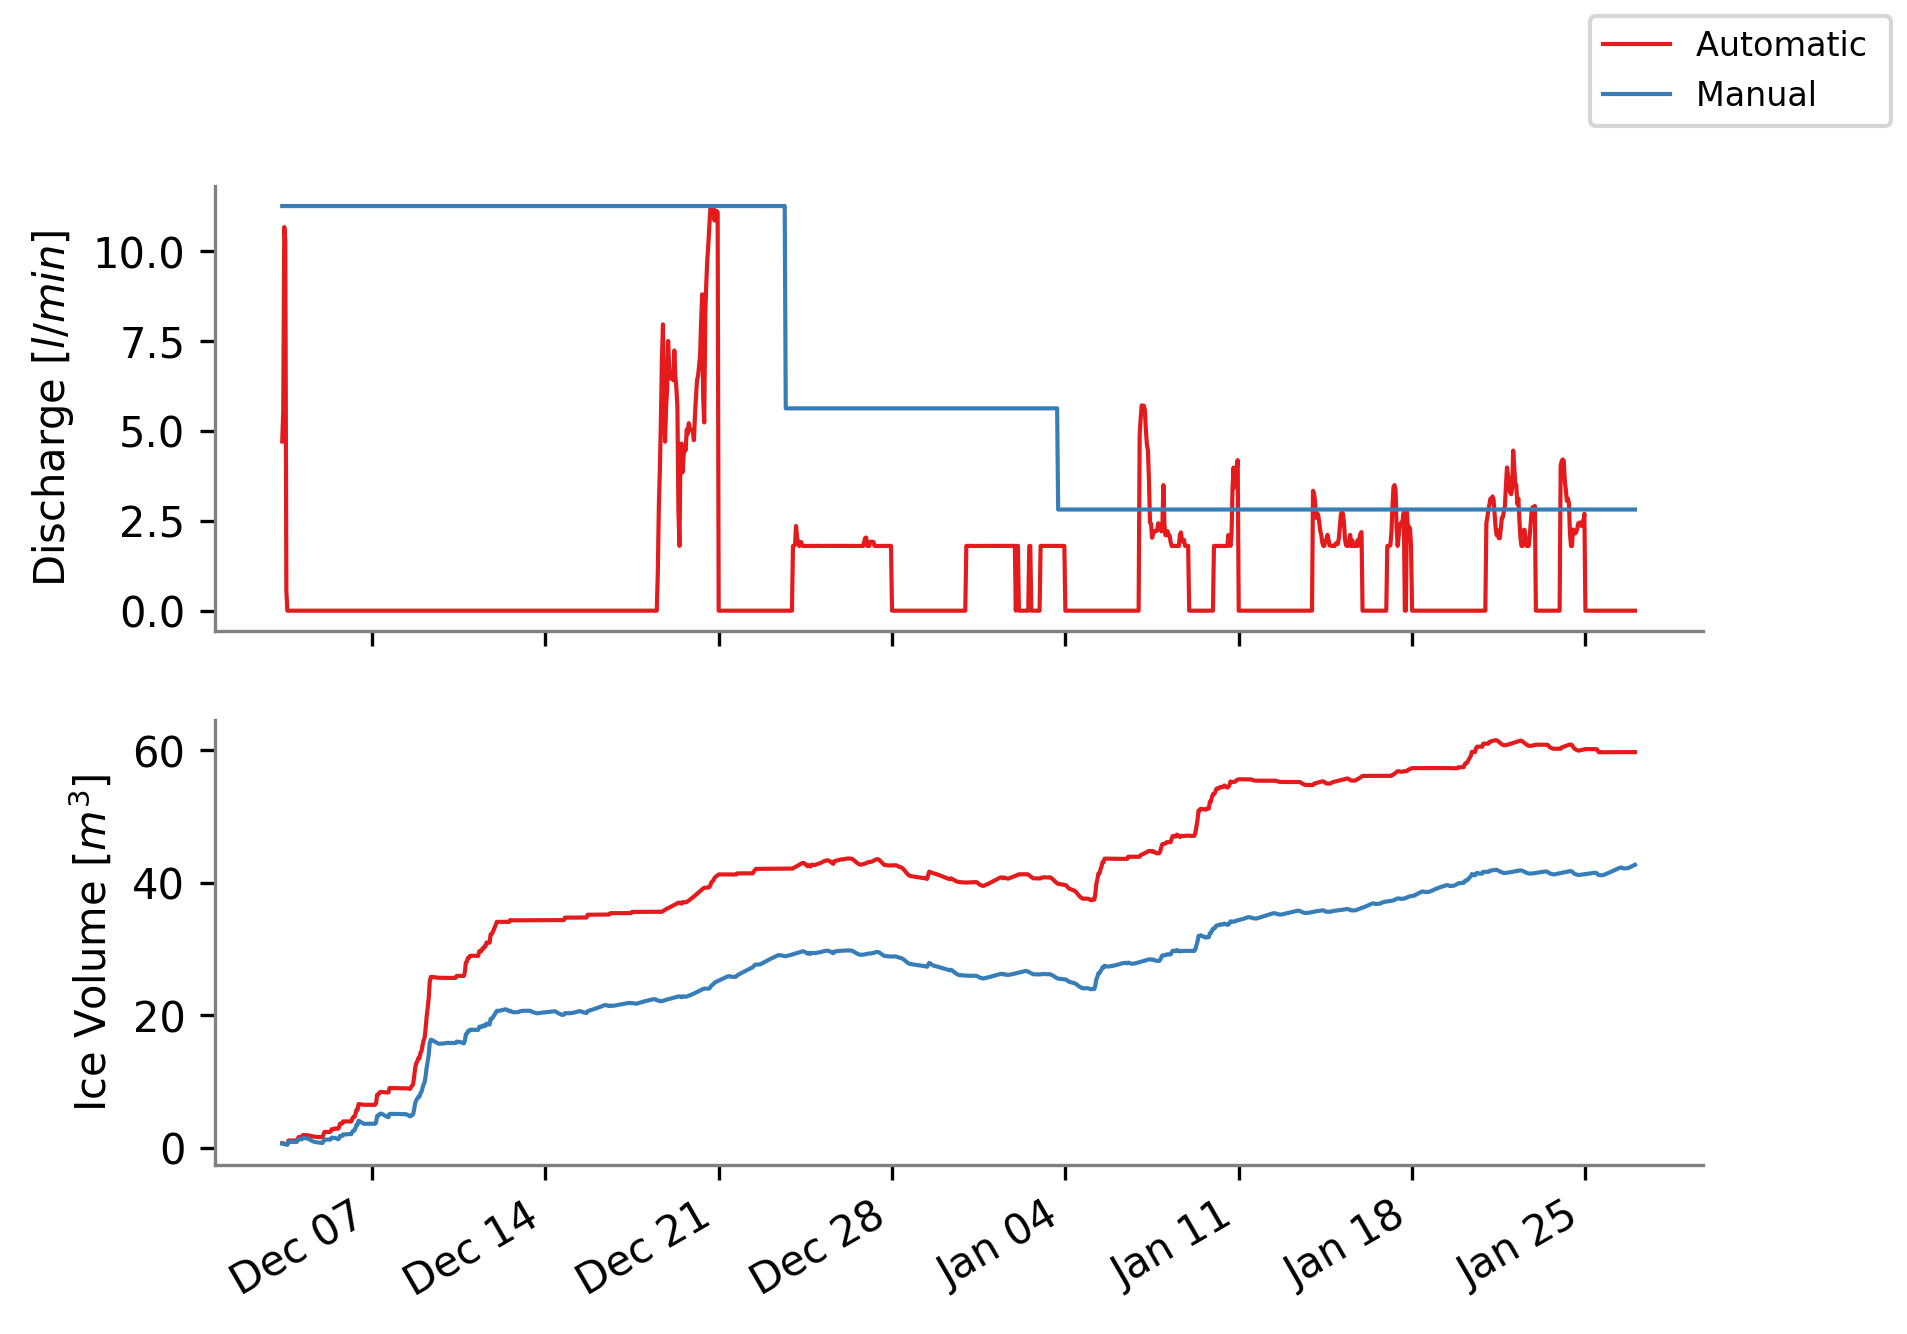
\includegraphics[width=\linewidth]{Figures/autovsmanual.png}
	\end{center}
	\caption{Comparison of discharge and ice volume between AIRs produced by automatic and manual methods. }
	\label{fig:old_icestupa}
\end{figure}

\subsection{Validation}

\section{Discussion}

\section{Conclusions}

\section{Appendix}

\subsubsection{Net Longwave radiation \texorpdfstring{$q_{LW}$}{Lg}} \label{sec:LW}
The net longwave radiation $q_{LW}$ is determined as follows:

\begin{equation}
	q_{LW}= \sigma \cdot \epsilon_a \cdot {(T_a+ 273.15)}^4 -\sigma \cdot \epsilon_{ice} \cdot {(T_{ice}+ 273.15)}^4
	\label{eqn:LW}
\end{equation}

where $T_a$ represents the measured air temperature, $\epsilon_a$ denotes the atmospheric emissivity $T_{ice}$
is the modelled surface temperature given in [$\degree C$], $\sigma=5.67\cdot10^{-8}\,Jm^{-2}s^{-1}K^{-4}$ is
the Stefan-Boltzmann constant and $\epsilon_{ice}$ is the corresponding emissivity value for the Icestupa
surface (0.97).

We approximate the atmospheric emissivity $\epsilon_a$ using the equation suggested by \cite{Brutsaert_1975},
considering air temperature and vapor pressure (Eqn. \ref{eqn:atm_e}). The vapor pressure of air over water and
ice was obtained using Eqn. \ref{eqn:vp}.  The expression defined in \cite{Brutsaert_1975} for clear skies
(first term in equation \ref{eqn:atm_e}) is extended with the correction for cloudy skies after
\cite{Brutsaert_1982} as follows:

\begin{equation}
	\epsilon_a=1.24 \cdot (\frac{p_{v,w}}{(T_a+273.15)})^{1/7}\cdot(1+0.22\cdot{cld}^2) \label{eqn:atm_e}
\end{equation}

with a cloudiness index $cld$, ranging from 0 for clear skies to 1 for complete overcast skies. 

The software assumes $T_{ice} = 0 \degree C$. This assumption overestimates $q_{LW}$ and thereby underestimates
the freezing rate.

\subsubsection{Turbulent fluxes} \label{sec:Qs}

The turbulent sensible $q_{S}$ and latent heat $q_{L}$ fluxes are computed with the following expressions
proposed by \cite{Garratt_1992}:

\begin{equation}
	q_{S}= c_{a} \cdot \rho_{a} \cdot p_{a}/p_{0,a} \cdot \frac{\kappa^2 \cdot v_a \cdot
		(T_a-T_{ice})}{{(\ln{\frac{h_{AWS}}{z_{0}}})}^2}
	\label{eqn:qs}
\end{equation}

\begin{equation}
	q_{L}= 0.623 \cdot L_s \cdot \rho_{a}/p_{0,a} \cdot \frac{\kappa^2 \cdot
	v_a(p_{v,w}-p_{v,ice})}{{(\ln{\frac{h_{AWS}}{z_{0}}})}^2}
\end{equation}

where $h_{AWS}$ is the measurement height above the ground surface of the AWS (around $2\,m$ for all sites),
$v_a$ is the wind speed in [$m\,s^{-1}$], $c_a$ is the specific heat of air at constant pressure (1010 J
$kg^{-1} K^{-1}$), $\rho_{a}$ is the air density at standard sea level (1.29 $kg m^{-3}$), $p_{0,a}$ is the air
pressure at standard sea level (1013 $hPa$), $p_{a}$ is the measured air pressure, $\kappa$ is the von Karman
constant (0.4), $z_{0}$ is the surface roughness (3 $mm$) and $L_s$ is the heat of sublimation (2848
$kJ\,kg^{-1}$).  The vapor pressure of air with respect to water ($p_{v,w}$) and with respect to ice
($p_{v,ice}$) was obtained using the formulation given in \cite{huang_2018} :

\begin{equation}
	\begin{split}
		p_{v,w}&=e^{\frac{(34.494 - \frac{4924.99}{T_{a} + 237.1})}{(T_a + 105)^{1.57} \cdot 100}} \cdot \frac{RH}{100} \\
		p_{v,ice}&=e^{\frac{(43.494 - \frac{6545.89}{T_{ice} + 278})}{(T_{ice} + 868)^{2} \cdot 100}} \\
	\end{split} \label{eqn:vp}
\end{equation}

The software ignores the $\mu_{cone}$ parameter thereby underestimating the turbulent fluxes.

\subsubsection{Net shortwave radiation \texorpdfstring{$q_{SW}$}{Lg}}
\label{sec:SW}

The net shortwave radiation $q_{SW}$ is computed as follows:

\begin{equation} q_{SW} = (1- \alpha_{ice}) \cdot ( SW_{direct} \cdot f_{cone} + SW_{diffuse})
\label{eqn:SW} \end{equation}

where $\alpha_{ice}$ is the bare ice albedo value (0.25); $SW_{global}$ is the global shortwave radiation and
$cld$ is a cloudiness index determined from historical weather data. The global shortwave radiation used is
modelled using the parametrisation proposed by \cite{Woolf_1968}.

The solar area fraction $f_{cone}$ of the ice structure exposed to the direct shortwave radiation depends on the
shape considered. Using the solar elevation angle $\theta_{sun}$, the solar beam can be considered to have a
vertical component, impinging on the horizontal surface (semicircular base of the AIR), and a horizontal
component impinging on the vertical cross section (a triangle). The solar elevation angle $\theta_{sun}$ used is
modelled using the parametrisation proposed by \cite{Woolf_1968}. Here we overestimate the impact of direct
solar radiation by assuming $h_{cone} = r_{cone} = r_{F}$. Accordingly, $f_{cone}$ is determined as follows:

\begin{equation}
	\begin{split}
		f_{cone}& =\frac{ cos \theta_{sun} + \pi \cdot sin \theta_{sun} }{2\sqrt{2} \cdot \pi }\\
	\end{split}
	\label{ eqn:f_{cone}}
\end{equation}

The software ignores the variations in the albedo and assumes it to be equal to that of ice to simplify the
model. This assumption overestimates the solar radiation absorption thereby underestimating the freezing rate.

\bibliographystyle{frontiersinSCNS_ENG_HUMS} \bibliography{refs}

\end{document}
